% CREATED BY DAVID FRISK, 2016
\chapter{Methods}
Chapter not finished

To be able to evaluate the performance of using Erlang to communicate in a WSN two prototypes need to be developed. From these prototypes data is going to be collected. After the data is collected, the data is going to be analysed to show when Erlang can be an alternative to a low-level language in a WSN. 

\section{Setup}
The product the company wants to develop is as mentioned in previous sections a video-based sensor network. A basic idea of how the network shall be constructed can be seen in Figure~\ref{fig:setup}. This is how the network is going to look like for the experiments, but the network design of the company’s final product must not necessary look like this. 

\begin{figure}[H]
\centering
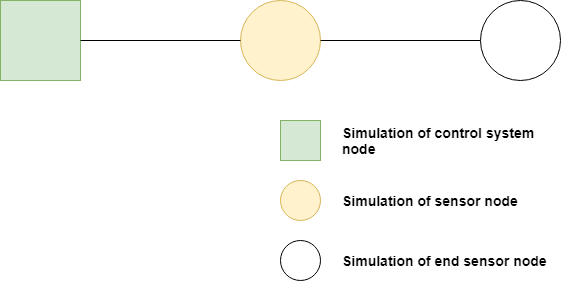
\includegraphics[scale=0.6]{figure/setup.png}
\caption{The company’s idea of the video-based sensor network.}
\label{fig:setup}
\end{figure}

There can be arbitrarily many sensor nodes in the network but there is no need for the network to be bigger than the one shown in Figure~\ref{fig:setup} for the investigation in this project. This is because the sensor that shall be investigated is a sensor that both receive data from another sensor and sends data to another device and that is fulfilled with the current network setup. 

The hardware to simulate the sensor that shall be investigated is going to be a Raspberry Pi, Freescale i.MX 6 or a similar development board. The only requirement is that the board can be made to communicate over the IEEE 802.15.4 standard and because the company has the Freescale I.MX 6 board it is going to be used if a ZigBee module can be acquired for it. For the nodes that simulate the control system and the end node the hardware platform does not matter. The only requirements are that they also can communicate over the IEEE 802.15.4 standard and that they have enough resources to not impact the sensor node that shall be investigated negatively. Therefore, they are going to be simulated with a PC and a USB IEEE 802.15.4 dongle.

There are many alternatives for operating system but because the company uses a basic Debian distribution in their other products and want to continue using it. It is this operating system that is going to be used for the sensor that is going to be investigated.

\section{Erlang}
The problem that needs to be solved in the case of the WSN that is part of this thesis is that it shall use direct device to device communication. The standard Erlang distribution facilities uses the TCP/IP protocol to communicate and this protocol as mention in previous section does not support direct device to device communication. The protocol that is going to be used instead is the ZigBee protocol and therefore support for this protocol needs to be added to Erlang. 

According to the Erlang homepage it is very hard to implement a new driver for the distribution carrier and it is therefore most likely that the solution is going to be to write a normal Erlang module to connect Erlang with the ZigBee protocol. It is possible that this is going to achieve slightly less performance but if it still good enough for someone to consider using Erlang, it is not going to be worse if a developer chooses to implement a new driver for the distribution carrier.

\section{Prototypes}
To be able to evaluate if Erlang is an alternative to a low-level language in developing the communication between sensors in a WSN, two prototypes shall be implemented. The first prototype is going to be developed by using the C language and the other with the Erlang language. 

The first step in the prototypes’ development process is to decide on a design. In this case the design is how the sensors in the network shall communicate. For example, shall a sensor ask for its child sensor’s data or shall the child sensor pass data to its parent without being asked for it.

After this first decision is made the approach to developing the prototypes are going to be the same iterative approach for both, where each step is going to be a small step towards completing the communication parts that are needed to evaluate if Erlang can manage the communication in the final product of the company. The choice of this iterative approach is to give the possibility to catch problems early and to only implement as much of the communication code as is needed to carry out the evaluation.

\section{Data collection}
From the two prototypes data is going to be collected for the purpose of evaluating the performance of using Erlang in a WSN. Both qualitative and quantitative data are going to be collected.

The qualitative data is going to be collected by counting how many lines of code the prototypes contains and by doing this a qualitative evaluation of the implementation effort of each prototype can be shown.

Quantitative data is going to be collected in multiple iteration, where each iteration has a different system load. System load is in this case the rate of communicated messages and the points of interest to measure are going to be power consumption, RAM utilization and CPU utilization. 

To measure the prototypes’ usage of RAM and CPU utilization, the \textit{ps} utility is going to be used. It is a Linux utility that reports information of running processes by reading the information from the virtual files in /proc filesystem. The last measurement that is going to be taken is the sensors power consumption. This is going to be done with a multimeter by running the application over a fixed time.  

\section{Evaluation}\label{sec:evaluation}
The evaluation part in this thesis is going to be to analyse the collected data based on the points in the following list to show when the use of Erlang could be a possibility for communication in a WSN.

\begin{itemize}
    \item Measure the overhead percentage between the Erlang solution relative to the C solution, by measuring the average iteration time of the application. 
    \item Calculate the percentage of how much capacity is lost or gained by using Erlang. How many messages can be sent with an Erlang solution compared to a C solution if the power budget, RAM utilization and CPU utilization is fixed respectively or if more than one hardware resource is fixed at the same time? 
    \item By subtracting idle power consumption, RAM utilization and CPU utilization of the Erlang VM from the performed measurements the minimum hardware requirements for running the application part of the sensor and the percentage overhead between the Erlang solution relative to the C solution can be calculated. 
\end{itemize}

By doing these analyzes, information is going to be collected and presented. This in turn gives someone that want to develop the communication between nodes in a WSN with Erlang a guideline for the hardware requirements. For example, if someone want to develop an WSN application and they have a fixed amount of RAM and some other process, they can then evaluate if there exist enough RAM for an Erlang communication solution.
